\documentclass[tikz,convert={density=300,outext=.png}]{standalone}
\begin{document}

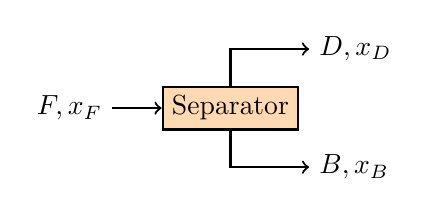
\begin{tikzpicture}
  %\draw[step=1cm,gray,very thin] (0,0) grid (10,7);
  \node[draw,thick,shape=rectangle,fill=orange!30] (Sep) at (3,2) {Separator};
  \draw[<-,thick] (Sep) -- ++(-1.5,0) node[left]{$F,x_F$};
  \draw[->,thick] (Sep) -- ++(0,0.75) -- ++(1,0) node[right]{$D,x_D$};
  \draw[->,thick] (Sep) -- ++(0,-0.75) -- ++(1,0) node[right]{$B,x_B$};
\end{tikzpicture}

\end{document}